\section{Models}
Different models and model architectures are the result of (restricted) computational resources, new ideas and algorithms, specific tasks, and so on. To approach our problem, we figured that experimenting with different models would likely point us into a direction of certain architectural features which work well with the data at hand.


\subsection{AlexNet}
\citeauthor{Krizhevsky2012} have presented their influential \emph{AlexNet} in \citeyear{Krizhevsky2012}. It consists of only five convolutional layers, some additional max-pooling layers and three fully connected layers at the end, so its structure is rather simple. Nonetheless, it is packed with more than 40 million trainable parameters (the fully connected layers at the end are very large), making it not exactly computationally cheap to train. An AlexNet was supposed to serve as our baseline model from which we wanted to build things up.


\subsection{EfficientNet}
We then implemented a pre-trained EfficientNet with custom top layer. The EfficientNet model family was first introduced in 2019 (\citeauthor{Tan2019}) with the idea of providing scalable CNN architectures. Their architecture is largely based on MobileNets inverted residual blocks, in which bottlenecks serve as in- and output of the residual connections \citep{Sandler2018}. Multiple networks of different size for image classification purposes were introduced, many achieving better results than state-of-the-art models like the MobileNet it built upon and ResNet while being significantly smaller in terms of depth, width, and image resolution \citep{Tan2019}. Two years later, a second, even more powerful and efficient generation was introduced: EfficientNetV2 \citep{Tan2021}. For our purposes, given the low input resolution of $224\times224$, the model of choice is the EfficientNetV2-B0 -- the smallest model of the ensemble. The model is pre-trained on ImageNet21k and we implemented a custom fully-connected layer at the end to match our classification task.


\subsection{InceptionNet}
For an additional comparison, we implemented yet another supposedly very efficiently designed CNN, the InceptionV3 as introduced by \citeauthor{Szegedy2015} in \citeyear{Szegedy2015}. Its computational low cost makes the Inception architecture an attractive choice when resources are limited, e.g. in mobile scenarios. The inception network was a milestone in the development of CNN classifiers. It achieved extremely high accuracies on the ImageNet dataset with InceptionV3 reaching $78.1\%$ accuracy.
The fundamental idea behind the inception network is the inception block. In a traditional convolutional neural network layer, the previous layer's output is the input of the next layer until the state of prediction is accomplished. The inception block takes apart the individual layers. The previous layer's output is passed to four different operations in parallel and their outputs is concatenated -- the network is made wider instead of deeper. The naïve approach consists of a $1\times1$ convolution layer, a $3\times3$ convolution layer and a $5\times5$ convolution layer followed by a maximum pooling operation and a concatenation layer. Due to the high computational cost especially of the $5\times5$ filter, the $1\times1$ filter is first added to the naïve inception module. This leads to a reduction in computations of $90\%$.
Additionally, the $1\times1$ convolutional filters allow learning cross-channel patterns across the depth of the input data. 

%picture of Convolution 
\begin{figure}[htb]
    \centering
    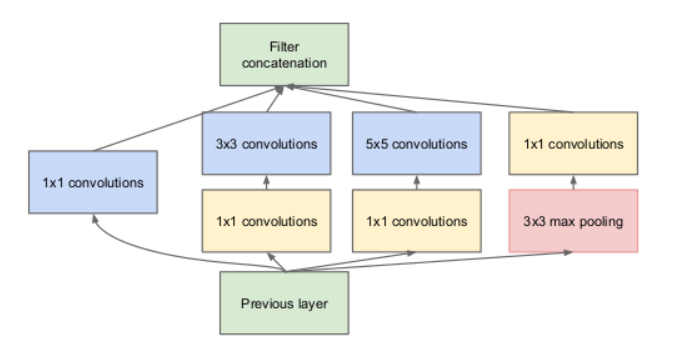
\includegraphics[width=7cm]{images/InceptionNet.jpg}
    \caption{Inception Block}
    \label{fig:incepblock}
\end{figure}